\documentclass[tikz,border=10pt]{standalone}
\usetikzlibrary{decorations.text}
\definecolor{mygray}{RGB}{208,208,208}
\definecolor{mymagenta}{RGB}{226,0,116}
\newcommand*{\mytextstyle}{\sffamily\normalfont\bfseries\color{black!85}}
\newcommand{\arcarrow}[3]{%
   % inner radius, middle radius, outer radius, start angle,
   % end angle, tip protusion angle, options, text
   \pgfmathsetmacro{\rin}{2.5}
   \pgfmathsetmacro{\rmid}{3.0}
   \pgfmathsetmacro{\rout}{3.5}
   \pgfmathsetmacro{\astart}{#1}
   \pgfmathsetmacro{\aend}{#2}
   \pgfmathsetmacro{\atip}{5}
   \fill[mygray, very thick] (\astart+\atip:\rin)
                         arc (\astart+\atip:\aend:\rin)
      -- (\aend-\atip:\rmid)
      -- (\aend:\rout)   arc (\aend:\astart+\atip:\rout)
      -- (\astart:\rmid) -- cycle;
   \path[
      decoration = {
         text along path,
         text = {|\mytextstyle|#3},
         text align = {align = center},
         raise = -1.0ex
      },
      decorate
   ](\astart+\atip:\rmid) arc (\astart+\atip:\aend+\atip:\rmid);
}
\newcommand{\barcarrow}[3]{%
   % inner radius, middle radius, outer radius, start angle,
   % end angle, tip protusion angle, options, text
   \pgfmathsetmacro{\rin}{3.9}
   \pgfmathsetmacro{\rmid}{4.4}
   \pgfmathsetmacro{\rout}{4.9}
   \pgfmathsetmacro{\astart}{#1}
   \pgfmathsetmacro{\aend}{#2}
   \pgfmathsetmacro{\atip}{5}
   \fill[mygray, very thick] (\astart+\atip:\rin)
                         arc (\astart+\atip:\aend:\rin)
      -- (\aend-\atip:\rmid)
      -- (\aend:\rout)   arc (\aend:\astart+\atip:\rout)
      -- (\astart:\rmid) -- cycle;
   \path[
      decoration = {
         text along path,
         text = {|\mytextstyle|#3},
         text align = {align = center},
         raise = -1.0ex
      },
      decorate
   ](\astart+\atip:\rmid) arc (\astart+\atip:\aend+\atip:\rmid);
}

\begin{document}
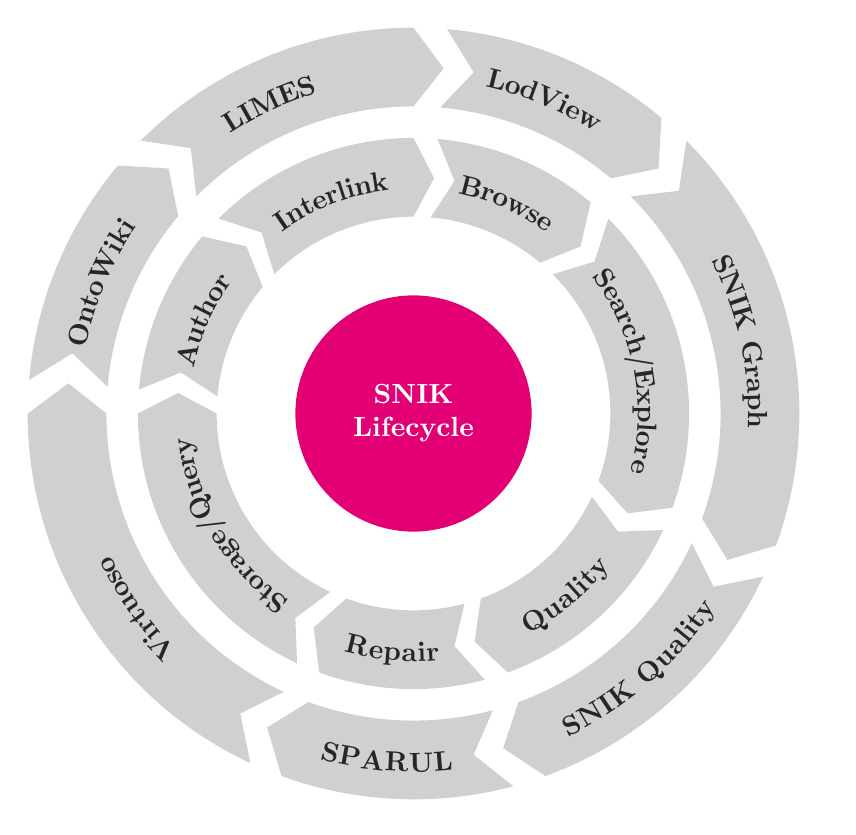
\begin{tikzpicture}
   \fill[even odd rule,mymagenta] circle (1.5);

   \node at (0,0) [
      font  = \mytextstyle,
      color = white,
      align = center
   ]{
      SNIK\\Lifecycle
   };
%   \arcarrow{ 85}{  3}{ Classification}
%   \arcarrow{ 85}{  3}{ Extraction}
%   \arcarrow{ 85}{  3}{ Transformation}
   \arcarrow{-120}{ -180}{~~~Storage/Query}
   \arcarrow{-190}{-220}{~~~Author}
   \arcarrow{-230}{-270}{~~~Interlink}

   \arcarrow{-280}{-310 }{~~~Browse}
   \arcarrow{-320}{-380 }{~~~Search/Explore}
   \arcarrow{-435}{-385 }{Quality~~~~}
 
  \arcarrow{-475}{-435}{Repair~~~~}

%   \arcarrow{ 85}{  3}{ Meta Model}
%   \arcarrow{ 85}{  3}{ Textbook Analysis}
%   \arcarrow{ 85}{  3}{ TARQL }
   \barcarrow{-120}{ -180}{Virtuoso}
   \barcarrow{-190}{-220}{~~~OntoWiki}
   \barcarrow{-230}{-270}{LIMES}
  
   \barcarrow{-280}{-310}{~~~LodView}
   \barcarrow{-320}{-380}{~~~SNIK Graph}
   \barcarrow{-435}{-385}{SNIK Quality~~~~}
   %\barcarrow{-435}{-385}{Validation Queries~~~~~~~}

  \barcarrow{-475}{-435}{SPARUL~~~~~}




\end{tikzpicture}





\end{document}

